\documentclass[conference]{IEEEtran}
\IEEEoverridecommandlockouts
\usepackage{cite}
\usepackage{amsmath,amssymb}
\usepackage{graphicx}
\graphicspath{{figures/}}
\usepackage{booktabs}
\usepackage{textcomp}
\usepackage[hidelinks]{hyperref}

\begin{document}

\title{Predicting Water Consumption and Tank Capacity\\for Mobile Car Washing}

\author{\IEEEauthorblockN{Naman Kumar, Ranu Raj, Vansh Rana, Priyanshu, Rudransh}
\IEEEauthorblockA{\textit{Module A7 --- Water and Supplies, Track A ``Service as a Service''}\\
\textit{BTech 7th Semester AI \& ML Thematic Assessment}}}

\maketitle

\begin{abstract}
Mobile car washing carries its water with it, so a crew's working day is bounded by tank
capacity rather than by demand. This module predicts per-job water consumption and converts
those predictions into operational capacity figures. We find that the variable driving
consumption is not the service tier a customer books but an add-on buried inside a delimited
item list, and that the strongest single predictor---how dirty the car is---is unobservable
until the crew arrives, forcing two separate models. A saturated cell-mean model reaches
$5.90 \pm 0.04$~L mean absolute error at booking time and $2.40 \pm 0.01$~L on site over ten
seeds, against an $11.15 \pm 0.06$~L baseline. Dividing tank capacity by mean consumption
overstates capacity badly: the resulting figures hold only 53--91\% of the time, and at a
95\% service level the defensible capacities are 2, 4 and 5 jobs for the 200, 280 and 350~L
vans. Choosing \emph{which} jobs to serve, an exact knapsack captures 13 points more revenue
than serving in booked order for under 4 points more jobs, while a greedy rule reaches 99\%
of that. Optimising on point predictions, however, doubles the rate at which plans overflow
the tank, from 5.9\% of crew-days to 11.9\%, because tight packing consumes the slack that
absorbed prediction error; planning on the interval's upper bound removes overflow entirely
for about ten points of throughput. Finally, we compare against published figures for
conventional car washing and find a mixed result: mobile washing uses roughly a quarter of
what home hose washing consumes, but nearly twice what a reclaim-equipped tunnel uses.
\end{abstract}

\begin{IEEEkeywords}
water consumption, demand prediction, knapsack, prediction intervals, service operations,
sustainability
\end{IEEEkeywords}

\section{Problem}

Doorstep sends crews to customers rather than customers to a wash bay. Every litre used at a
job was loaded into a van beforehand, which makes two questions operational rather than
academic: how much water will a given job consume, and how many jobs can a van serve before
it must refill. The second question is what constrains scheduling, and it cannot be answered
well without the first. A module that predicts consumption accurately but reports capacity as
a single number will mislead whoever schedules the day.

\section{Related Work}

\subsection{What a car wash consumes}
Monney et al.~\cite{monney2020carwash} give empirical estimates of water consumption and
pollution loads across the commercial carwash industry, establishing that per-vehicle
consumption must be measured rather than assumed. Maciejewska and
Reizer~\cite{maciejewska2025carbon} compare four professional wash types and find carbon
footprints from 0.88~kg CO\textsubscript{2} (hand wash, gas heating) to 4.46~kg
CO\textsubscript{2} (rollover, electric heating), concluding that wash \emph{type} dominates
the footprint. Zaneti et al.~\cite{zaneti2013reuse} audit a full-scale reclamation plant over
22 weeks and report almost 70\% reclamation, needing fewer than 40~L of fresh water per wash.
Together these frame our comparison: the spread across facility types is far wider than the
spread within one, so a single ``conventional car wash'' figure would be meaningless.
Zaneti et al. also corroborate our result from outside our data---at under 40~L fresh per
wash, a reclaim-equipped facility uses less than our measured 55.7~L, and a mobile van cannot
reclaim because the water leaves with it.

\subsection{Predicting water demand}
Donkor et al.~\cite{donkor2014demand} review urban water-demand forecasting and find that
method complexity is a weak predictor of accuracy: simple models frequently match
sophisticated ones once the right variables are present. Our finding that three model
families are indistinguishable once the interior add-on is parsed is the same observation at
job scale.

\subsection{Deciding under an uncertain capacity constraint}
Kleywegt and Papastavrou~\cite{kleywegt1998dynamic,papastavrou1996deadlines} formalise the
dynamic and stochastic knapsack, where item sizes are random and capacity may be violated.
Han et al.~\cite{han2015chance} treat the chance-constrained binary knapsack, replacing a hard
capacity constraint with one that must hold at a stated probability. This is our tank problem:
the service-level formulation used here is that chance constraint solved empirically by
resampling rather than analytically, and this literature is why we report capacity at a
service level rather than as a single number.

\subsection{Why optimising on predictions can backfire}
Elmachtoub and Grigas~\cite{elmachtoub2022spo} show that minimising prediction error is not
the same as minimising decision cost, and that a better-fitting model can yield worse
decisions once its output is fed to an optimiser. Our result in
Section~\ref{sec:selection}---that an exact knapsack doubles the tank-overflow rate relative
to serving in booked order---is an empirical instance of this. We note one difference: their
setting places uncertainty in the objective, whereas ours is in the constraint.

\subsection{Turning a prediction into a safe input}
Lei et al.~\cite{lei2018conformal} give distribution-free prediction intervals with
finite-sample coverage from a held-out calibration split; Koenker and
Bassett~\cite{koenker1978quantiles} establish quantile regression as the alternative route to
the same quantity. We use the split-calibration construction, and our decision to plan
against the interval's upper bound rather than its centre is the practical consequence.

\subsection{Routing and capacity in service fleets}
Braekers et al.~\cite{braekers2016vrp} classify the vehicle routing literature and note that
most capacitated variants treat demand as deterministic. This module supplies the per-job
distribution that a stochastic-demand routing model would require.

\subsection{What we do not borrow}
No study we found models water consumption at the level of an individual mobile wash job, and
none reports the interaction structure we observe---dirtiness multiplying a vehicle-size base
while an interior add-on contributes a constant. The per-job model here is built from the data
rather than adapted from prior work.

\section{Data}

The Doorstep simulated dataset~\cite{doorstep2026dataset} covers 1 January 2024 to 31 December
2025. This analysis uses \texttt{jobs\_done.csv} (39,302 completed jobs), \texttt{bookings.csv}
for booking-time attributes, and \texttt{vehicles.csv} for tank capacities.

The dataset is simulated, generated with a fixed seed, and contains no real personal data.
Results describe that simulation, not real operations.

The target \texttt{water\_litres} has mean 55.68~L, standard deviation 13.60~L and range
22.8--103.6~L. \texttt{jobs\_done} is complete, has no duplicate rows, and joins one-to-one
with the completed bookings. The duplicate-row glitch planted in \texttt{bookings} for another
module never reaches \texttt{jobs\_done}. The only missing values in the working frame are 314
blank \texttt{total\_price} cells (0.8\%, blank by design), which are not used as a feature.

\section{Exploratory Findings}

Four findings determined the modelling approach.

\textbf{The service tier is a decoy.} All five \texttt{slot\_type} values average between 54.9
and 55.8~L. The variable that matters is the \texttt{interior\_clean} add-on, which appears
inside the pipe-delimited \texttt{items} string on 27.9\% of jobs and adds $+18.0$~L. It is
sold across every slot type (Fig.~\ref{fig:decoy}), so a feature set built from \texttt{slot\_type} alone misses the
second-largest effect available at booking time. Extracting it requires parsing a string field
rather than reading a column, which is precisely why it is easy to miss.

\begin{figure}[t]
\centering
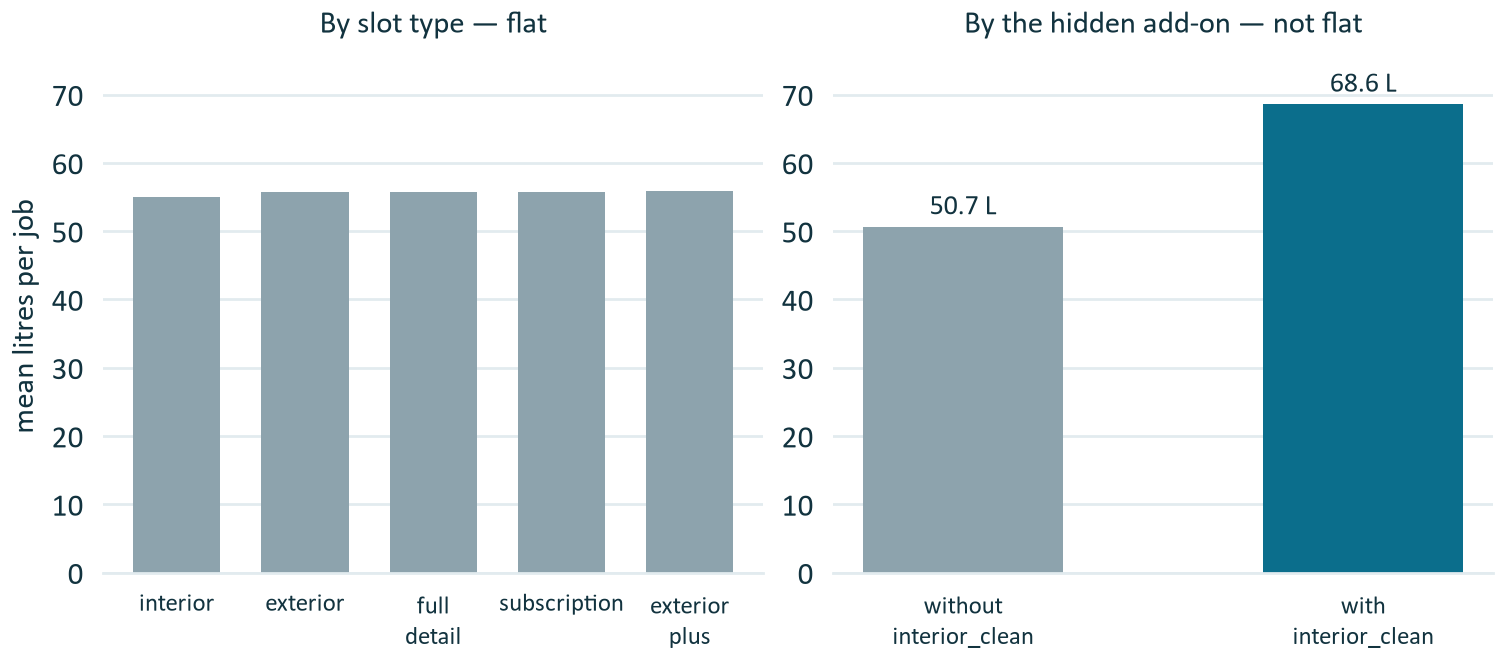
\includegraphics[width=\columnwidth]{slot_vs_addon.png}
\caption{Mean water per job by service tier (left) against the same jobs split by the \texttt{interior\_clean} add-on parsed from the item string (right). The tier a customer books is flat; the add-on hidden inside it is not.}
\label{fig:decoy}
\end{figure}

\textbf{Dirtiness multiplies; the add-on adds.} Dirtiness scales the vehicle-size base by
1.00 / 1.18 / 1.35 / 1.53, identically across all three vehicle sizes (Fig.~\ref{fig:form}), while
\texttt{interior\_clean} contributes a flat $+18$~L regardless of size or dirtiness. A purely
additive linear model is therefore mis-specified and needs a size $\times$ dirtiness
interaction.

\begin{figure}[t]
\centering
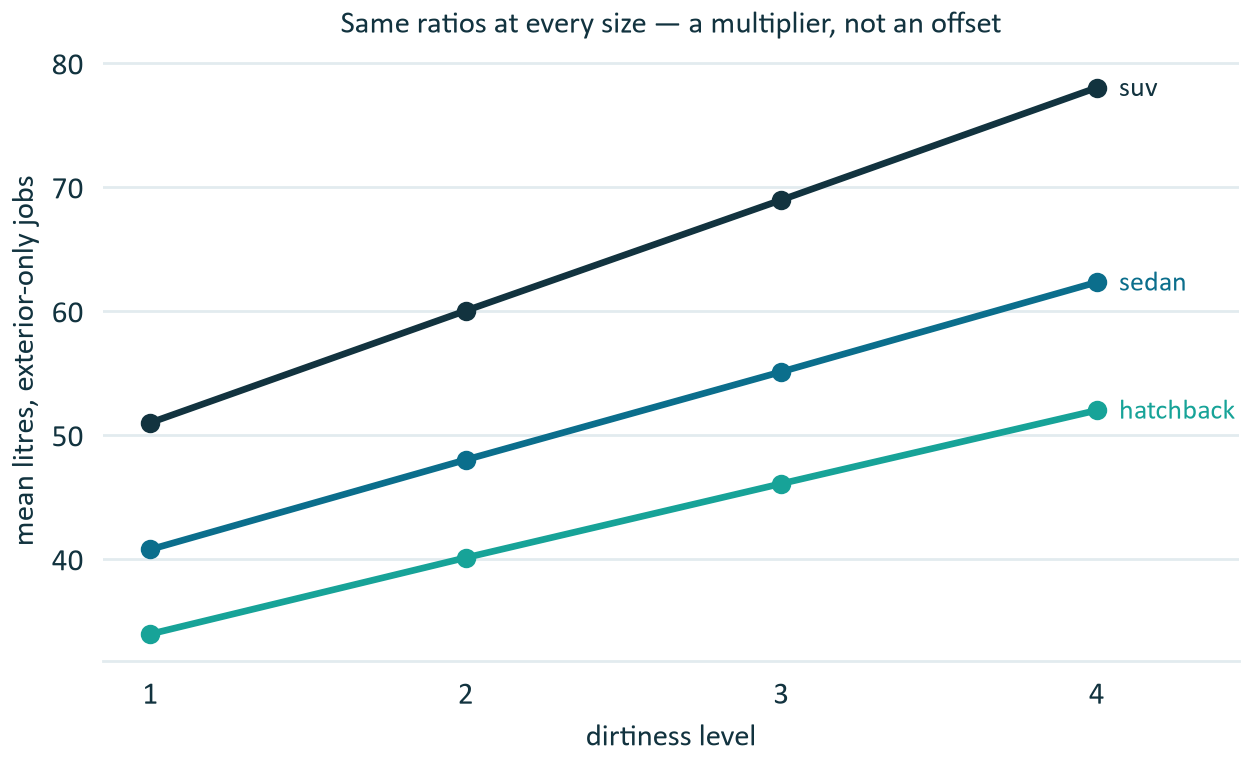
\includegraphics[width=\columnwidth]{functional_form.png}
\caption{Mean water by vehicle size and dirtiness level. The curves are parallel in ratio rather than in difference: dirtiness scales a size-dependent base by the same 1.00 / 1.18 / 1.35 / 1.53 factors for every vehicle size, which is why an additive model is mis-specified.}
\label{fig:form}
\end{figure}

\textbf{Dirtiness is unknowable before arrival.} \texttt{dirtiness\_level} is recorded when the
crew reaches the vehicle. It is uncorrelated with rainfall ($-0.007$) and temperature
($+0.001$), flat across calendar months, and within-customer variation (sd 0.89) swamps
between-customer variation (sd 0.28)---it behaves as an independent draw. This is the central
constraint of the module: the best available predictor is structurally unavailable when the
prediction is most useful.

\textbf{The noise floor is additive and uniform.} Within an exact feature cell, jobs scatter
with sd $\approx 3.0$~L, equally for interior and exterior jobs. The spread does not grow with
the cell mean, so the noise is additive rather than proportional. This sets a hard floor on
achievable error.

\section{Method}

\subsection{Two prediction stages}
Because dirtiness arrives late, two models are trained on disjoint feature sets: a
\emph{planning} stage using vehicle size and the interior add-on, available when the booking is
taken; and an \emph{on-site} stage adding dirtiness and its size interaction, available once
the crew has seen the car. Using dirtiness in the planning-time model would be leakage and
would produce a model that benchmarks well and fails in deployment. Post-job columns
(\texttt{duration\_minutes}, \texttt{late\_minutes}, \texttt{rating}, \texttt{revenue}) are
outcomes rather than inputs and are excluded from both stages by construction, a property
enforced by a test rather than by convention.

\subsection{Model families and seeds}
Three families were compared at each stage against two baselines: a global mean, a
per-vehicle-size group mean, a saturated cell mean, linear regression with the size $\times$
dirtiness interaction, and gradient boosting. Every split-dependent number in this paper is the
average over \textbf{ten seeds}, reported with its standard deviation. A single split would not
distinguish these models from one another, as Section~\ref{sec:accuracy} shows.

\subsection{Prediction intervals}
Point estimates are inadequate for capacity planning, so each scenario carries a 90\% interval
from residual quantiles, calibrated on a split disjoint from both the fitting and test splits
(a 60/20/20 arrangement) following~\cite{lei2018conformal}. Calibrating and measuring coverage
on the same rows would report the nominal level back by construction.

\subsection{Tank capacity and refills}
Capacity is evaluated by resampling observed per-job consumption 20,000 times and asking how
often $n$ jobs actually fit (Fig.~\ref{fig:feasibility}), rather than dividing capacity by the mean. Refills are counted by
walking each crew-day in arrival order and topping up before any job the remaining water cannot
cover, assuming each day starts with a full tank.

\subsection{Choosing the best set of jobs}
Given a crew-day's bookings and a tank, the module selects a subset by three methods: serving in
booked order until the tank cannot cover the next job (the manager's default, and the baseline),
greedily taking the highest revenue per litre, and an exact 0/1 knapsack solved by dynamic
programming over integer decilitres. Revenue is the objective rather than a feature---it equals
the booking's quoted \texttt{total\_price}, so it is known when the plan is made and is never
used to predict water. Each method runs from three planning bases: actual consumption (an oracle
no planner can reach), the planning model's point estimate, and the upper end of its 90\%
interval. Selection uses the planning basis; feasibility is judged against actual consumption.

\section{Results}

\subsection{Prediction accuracy}
\label{sec:accuracy}

\begin{table}[t]
\caption{Mean absolute error and $R^2$, mean $\pm$ sd over ten seeds}
\label{tab:accuracy}
\centering
\small
\begin{tabular}{llcc}
\toprule
Stage & Model & MAE (L) & $R^2$ \\
\midrule
Baseline & global mean & $11.152 \pm 0.062$ & $-0.000$ \\
Baseline & vehicle-size mean & $8.922 \pm 0.067$ & $0.358 \pm 0.006$ \\
Planning & cell mean & $\mathbf{5.897 \pm 0.038}$ & $0.715 \pm 0.004$ \\
Planning & linear & $5.897 \pm 0.038$ & $0.715 \pm 0.004$ \\
Planning & gradient boosting & $5.896 \pm 0.038$ & $0.715 \pm 0.004$ \\
On-site & cell mean & $\mathbf{2.397 \pm 0.014}$ & $0.952 \pm 0.001$ \\
On-site & linear & $2.397 \pm 0.015$ & $0.952 \pm 0.001$ \\
On-site & gradient boosting & $2.397 \pm 0.014$ & $0.952 \pm 0.001$ \\
\bottomrule
\end{tabular}
\end{table}

Table~\ref{tab:accuracy} and Fig.~\ref{fig:spread} report the comparison. \begin{figure}[t]
\centering
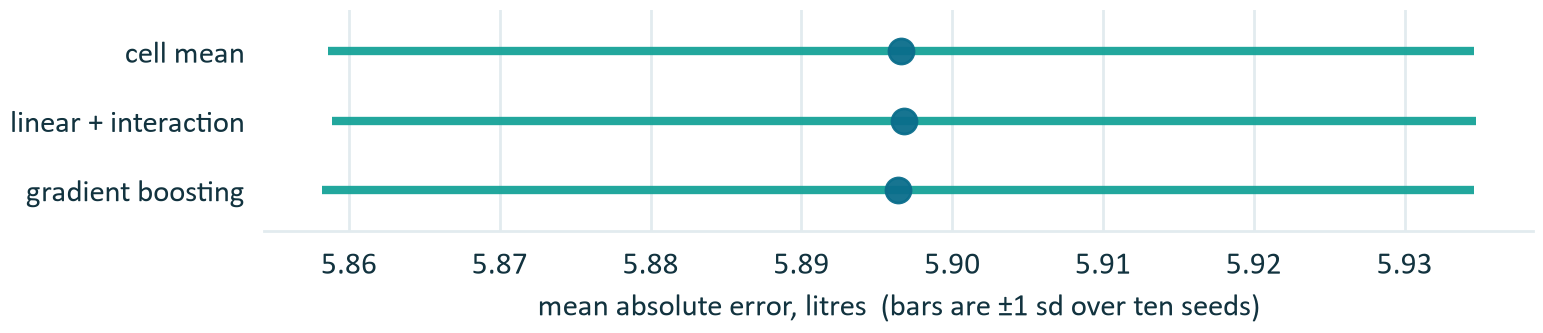
\includegraphics[width=\columnwidth]{model_spread.png}
\caption{Mean absolute error for the three planning-stage families, with bars at $\pm 1$ standard deviation over ten seeds. The three means differ by 0.001~L while each bar spans roughly 0.08~L, so the families cannot be separated by this evidence.}
\label{fig:spread}
\end{figure}

The three families are indistinguishable, and the ten-seed spread is what makes that statement
defensible rather than merely apparent: they differ by 0.001~L while the seed-to-seed standard
deviation is 0.038~L at planning time---the noise between splits is roughly forty times the gap
between models. Reported from one split, the ranking between them would be an artefact of which
rows happened to land in the test set.

This is informative rather than disappointing. The underlying structure is a small,
fully-populated contingency table, with 6 cells at planning time and 24 on site, each supported
by between 285 and 4,307 observations. Once the correct features are present there is nothing
left for a flexible model to find. Model selection therefore takes the simplest family within
1\% of the best seed-averaged MAE rather than the raw minimum, which selects the cell mean at
both stages; selecting by raw argmin would have shipped a gradient-boosting ensemble for a
0.0003~L improvement.

The on-site RMSE of 3.00~L sits at the noise floor identified in exploration, meaning the
on-site model extracts essentially all available signal. Measured interval coverage is
$0.8985 \pm 0.0053$ at planning time and $0.9000 \pm 0.0052$ on site, against a 0.90 nominal
level. The gap between stages quantifies the cost of not knowing dirtiness: MAE roughly doubles,
from 2.40~L to 5.90~L, and the interval widens from about $\pm 5$~L to about $\pm 12$~L.

\subsection{Tank capacity}

\begin{table}[t]
\caption{Maximum jobs per tank by service level}
\label{tab:capacity}
\centering
\small
\begin{tabular}{lccccc}
\toprule
Vehicle & Cap. & Mean-based & Fits & 95\% & 99\% \\
\midrule
small\_van & 200~L & 3 jobs & 90.9\% & \textbf{2} & 2 \\
ev\_van & 280~L & 5 jobs & 53.4\% & \textbf{4} & 3 \\
large\_van & 350~L & 6 jobs & 69.6\% & \textbf{5} & 4 \\
\bottomrule
\end{tabular}
\end{table}

The mean-based figures are not merely imprecise, they are wrong in a specific and damaging
direction. Loading an EV van for the five jobs that dividing 280~L by 55.68~L suggests leaves
the crew short roughly once every two days. Per-job consumption has a standard deviation of
13.60~L and a maximum of 103.6~L, and summing several draws from that distribution produces a
spread that mean arithmetic discards entirely. \textbf{A capacity figure quoted without a
service level is not a usable number.} These capacities are stable: repeating the resampling
under ten different seeds returns the same 2 / 4 / 5 jobs at every service level.

\begin{figure}[t]
\centering
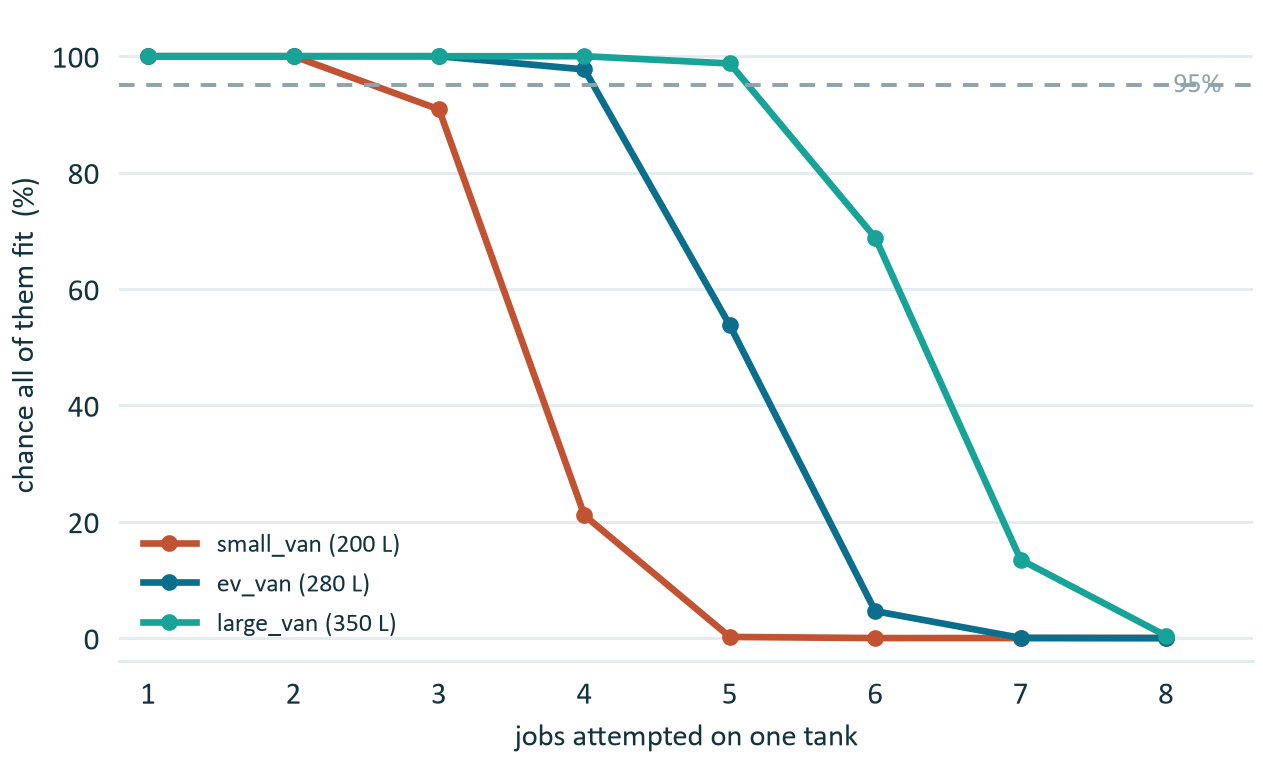
\includegraphics[width=\columnwidth]{tank_feasibility.png}
\caption{Probability that $n$ jobs fit in one tank, by vehicle, from 20,000 resampled crew-days. The horizontal line marks the 95\% service level; where each curve crosses it gives the defensible capacity in Table~\ref{tab:capacity}.}
\label{fig:feasibility}
\end{figure}

\subsection{Refill frequency}

\begin{figure}[t]
\centering
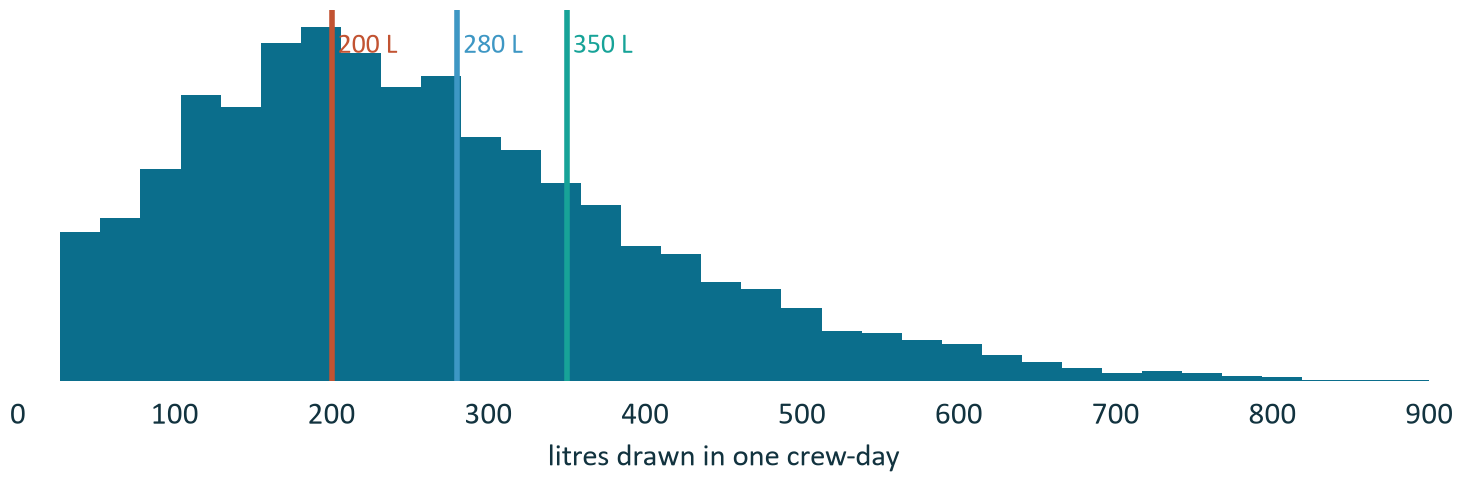
\includegraphics[width=\columnwidth]{crew_day_load_light.png}
\caption{Water drawn per crew-day across 8,342 crew-days, with the three tank capacities marked. Most of the distribution lies to the right of the 200~L van, and a substantial tail lies beyond all three.}
\label{fig:load}
\end{figure}

A single jobs-per-tank figure conceals the real constraint. Crews average 4.7 jobs and 262~L per
day across 8,342 crew-days, with a 95th percentile of 544~L---beyond every tank in the fleet (Fig.~\ref{fig:load}).
Mean refills per crew-day are 0.88, 0.45 and 0.26 for the 200, 280 and 350~L vans; 20.9\% of
small-van days need two or more. Refilling is normal operation, not an exception. For fleet
planning this reframes tank size: the difference between a 200~L and a 350~L van is not simply
jobs per fill but 0.88 against 0.26 interruptions per working day, each costing travel time to a
water source.

\subsection{The best set of jobs}
\label{sec:selection}

\begin{table}[t]
\caption{Job selection: share of all jobs and revenue captured, and share of crew-days whose
plan exceeded the tank}
\label{tab:selection}
\centering
\small
\begin{tabular}{llccc}
\toprule
Basis & Method & Jobs & Revenue & Overflow \\
\midrule
\multicolumn{5}{l}{\emph{200~L van}} \\
oracle & booked order & 59.3\% & 58.5\% & 0.0\% \\
oracle & exact knapsack & 63.1\% & 71.7\% & 0.0\% \\
point & booked order & 59.0\% & 58.3\% & 5.9\% \\
point & value density & 61.1\% & 70.3\% & 8.1\% \\
point & exact knapsack & 61.8\% & 71.0\% & \textbf{11.9\%} \\
safe & exact knapsack & 52.3\% & 61.9\% & \textbf{0.0\%} \\
\midrule
\multicolumn{5}{l}{\emph{280~L van}} \\
point & exact knapsack & 78.8\% & 84.8\% & 10.5\% \\
safe & exact knapsack & 68.9\% & 77.0\% & 0.0\% \\
\midrule
\multicolumn{5}{l}{\emph{350~L van}} \\
point & exact knapsack & 87.8\% & 91.6\% & 7.0\% \\
safe & exact knapsack & 79.4\% & 85.4\% & 0.0\% \\
\bottomrule
\end{tabular}
\end{table}

Table~\ref{tab:selection} gives three results, in increasing order of interest.

\textbf{Optimising by value buys revenue, not jobs.} On the 200~L van the exact knapsack
captures 13.2 points more revenue than booked order for only 3.8 points more jobs, by preferring
jobs worth more per litre. The operational gain is in what is served, not how much.

\textbf{Exact optimisation barely beats greedy.} Value-density greedy reaches 70.9\% of revenue
against the knapsack's 71.7\%---about 99\% of optimal. Crew-days contain a median of four jobs,
and knapsack instances that small are rarely hard. The exact solver is worth building in order
to \emph{know} the greedy rule is sufficient; it is not worth deploying over it.

\textbf{Better optimisation makes the plan more fragile.} This is the result we did not expect.
Planning on point predictions, booked order overflows the 200~L tank on 5.9\% of crew-days, but
the exact knapsack overflows on 11.9\%---optimising doubles the failure rate. Packing a tank to
its limit consumes exactly the slack that absorbed prediction error; a loose plan is
accidentally robust. Planning instead on the upper end of the 90\% interval removes overflow
entirely, at a cost of roughly ten points of jobs and revenue. That trade is the module's
central practical claim: an optimiser fed point estimates optimises the mean day and fails the
bad one. The interval is not decoration on the prediction, it is what makes the optimiser safe
to use. This is the decision-versus-prediction gap of~\cite{elmachtoub2022spo}, reached
empirically and with the uncertainty located in the constraint rather than the objective.

\subsection{Sustainability comparison}

Doorstep draws no reclaimed water---a mobile van cannot recover what it sprays---so its 55.7~L
per job is entirely freshwater and compares directly against published freshwater figures. It
uses 22--25\% of what a friction conveyor without reclaim, an in-bay automatic without reclaim,
or a home hose left running consumes~\cite{epa2012watersense,epa_hose}; 33\% and 49\% of the
measured in-bay and conveyor fleet averages~\cite{ica2018water}; and lands level with a
self-service wand bay at 98\%. Against reclaim-equipped facilities it is \emph{worse}: 184\% of
an in-bay automatic with reclaim and 189\% of a friction conveyor with
reclaim~\cite{epa2012watersense}, consistent with the under-40~L figure
of~\cite{zaneti2013reuse}.

The honest reading is mixed. Mobile washing uses roughly a quarter of what home hose washing and
unreclaimed facilities consume, but a reclaim-equipped tunnel uses about half what Doorstep does
per car, and that gap is structural: reclaim requires capturing runoff, which a van parked on a
customer's driveway cannot do. \textbf{The defensible claim is against home washing and against
unreclaimed or typical operating facilities---not against best-in-class fixed sites.} Two
caveats are carried in the data rather than hidden: the home-hose figure is derived, since the
EPA publishes a flow rate rather than a per-wash total, and the industry figures come from a
body reporting on its own sector.

\section{Limitations}

\begin{itemize}
\item \textbf{Simulated data.} Every figure describes a generated dataset with known structure.
\item \textbf{The noise floor may be an artefact.} The uniform $\approx 3.0$~L within-cell
scatter is a property of the generator; real jobs would likely show heteroscedasticity.
\item \textbf{Job selection assumes a known, droppable day.} Bookings are treated as known in
advance and free to drop. Refusing a confirmed booking carries a customer cost that is not
priced, so the selection figures are an upper bound.
\item \textbf{Selection plans one tank-load and ignores refills.} A combined model would decide
when to refill and what to serve jointly.
\item \textbf{Revenue is the only objective.} A real operation would weigh retention, fairness
across crews, and travel distance alongside it.
\item \textbf{Refill counts assume water is always available}, with no travel time to a source
and no queueing; refills are counted, not costed.
\item \textbf{The sustainability benchmarks are US figures} applied to an Indian operating
context, and sources define freshwater use differently. The table reports the definitional split
rather than averaging across it.
\end{itemize}

\section{Conclusions}

The module's most transferable finding is methodological. The largest available predictor was
hidden inside a delimited string rather than exposed as a column, and the strongest predictor
overall was unavailable at prediction time. Neither is visible from a correlation matrix, and
both determined the shape of the solution more than any modelling choice did. Once the features
were right, three model families of very different capacity performed identically---suggesting
that effort spent on feature semantics returned more than effort spent on model selection would
have, an observation that matches~\cite{donkor2014demand} at a different scale.

The optimisation result points the same way. The exact knapsack was worth building mainly to
establish that a greedy rule already reaches 99\% of it, and the more consequential finding was
not about solution quality at all: optimising against point predictions doubled the rate at
which plans overflowed the tank. A better optimiser made the operation less reliable, because
packing to the limit spends the slack that had been quietly absorbing prediction error.
Uncertainty and optimisation cannot be treated as separate concerns---the optimiser has to
consume the interval, not the point.

Operationally, we recommend that capacity be quoted as an interval with a stated service level,
that refill frequency rather than jobs per tank be treated as the planning quantity, and that any
selection run against the interval's upper bound rather than its centre.

\section*{Reproducibility}

All results regenerate with \texttt{python src/train.py} followed by
\texttt{python -m pytest tests -q}. Seed 7 matches the dataset generator; the ten-seed sweep uses
seeds 0--9. Code, outputs and the experiment log are in the module repository.

\bibliographystyle{IEEEtran}
\bibliography{refs}

\end{document}
